\section{Mobil Uygulama}
\label{CH:Uygulama}

\subsection{Modelin telefona aktarılması}

Eğitilen modeller LiteRT (\texttt{.tflite}) biçimine dönüştürülmüştür~\cite{LiteRT}.
PyTorch'tan doğrudan dönüşüm aracı (\texttt{ai-edge-torch}) eğitim bilgisayarına
kurulamadığı için modeller Keras'ta aynı katmanlarla yeniden kurulmuş ve ağırlıklar
birebir taşınmıştır. BiGRU'da PyTorch'un kapı sırası $(r, z, n)$ Keras'ın $(z, r, h)$
sırasına çevrilmiştir. 1B-CNN + Transformer'da ise şu farklara dikkat edilmiştir:
evrişim ağırlıklarının eksen sırası, 2 adımlı evrişimde Keras'ın \texttt{same} dolgusunun
sağa fazladan sıfır eklemesi (açık dolgu ve \texttt{valid} ile çözülmüştür), normalizasyon
katmanlarının epsilon değeri ($10^{-5}$) ve GELU'nun tam (erf) sürümü. Keras ile PyTorch
çıktıları arasındaki en büyük fark $7\times10^{-6}$ olarak ölçülmüştür.

Dönüştürülen modellere dinamik aralık int8 nicemleme uygulanmıştır: ağırlıklar 8 bit
saklanmakta, hesaplamalar kayan noktada yapılmaktadır. Sonuçlar
Tablo~\ref{tab:donusum} içinde verilmiştir.

\begin{table}[H]
\centering
\caption{LiteRT dönüşümü sonrası boyut ve test doğruluğu (3.741 test videosu; son sütun PyTorch modeliyle aynı tahmin oranı)}
\label{tab:donusum}
\small
\begin{tabular}{@{}llrrr@{}}
\toprule
\textbf{Model} & \textbf{Biçim} & \textbf{Boyut (MB)} & \textbf{Test (\%)} & \textbf{Aynı tahmin (\%)} \\
\midrule
BiGRU & fp32 & 9,43 & 88,00 & 100,0 \\
BiGRU & int8 & 3,19 & 88,00 & 99,5 \\
1B-CNN + Transformer & fp32 & 5,95 & 89,79 & 100,0 \\
1B-CNN + Transformer & int8 & \textbf{1,61} & \textbf{89,82} & 99,6 \\
\bottomrule
\end{tabular}
\end{table}

Nicemleme doğruluğu düşürmemiş, 1B-CNN + Transformer modelinin int8 sürümü BiGRU'nun
yarısı boyutunda kalmıştır. Uygulamada bu sürüm kullanılmaktadır.

\subsection{Mimari}

Uygulama Flutter ile yazılmış, kamera ve hesaplama işleri Kotlin tarafında
tutulmuştur (Şekil~\ref{fig:mimari}). Her kareyi Flutter ile Kotlin arasında taşımak
kare hızını belirgin biçimde düşüreceği için kamera görüntüsü, MediaPipe ve model
çıkarımı tamamen Kotlin'de çalışmaktadır. Flutter tarafına yalnızca yarım saniyede bir
özet bilgiler (kare hızı, görünen el sayısı) ve tanıma sonuçları olay kanalı
(\textit{event channel}) üzerinden gelmektedir.

\begin{figure}[H]
\centering
\resizebox{\textwidth}{!}{%
\begin{tikzpicture}[
  kutu/.style={draw, rounded corners, align=center, minimum height=1.0cm, minimum width=2.2cm, font=\small},
  ok/.style={-{Latex}, thick}]
\node[kutu] (kam) {CameraX\\(analiz görüntüsü)};
\node[kutu, right=0.5cm of kam] (mp) {MediaPipe\\el + gövde};
\node[kutu, right=0.5cm of mp] (on) {Normalizasyon\\$64\times100$};
\node[kutu, right=0.5cm of on] (lr) {LiteRT\\int8 model};
\node[kutu, below=1.2cm of lr] (seg) {Eşik ve\\segmentleme};
\node[kutu, left=0.5cm of seg, minimum width=5.2cm] (fl) {Flutter arayüzü\\Tanı · Metin · İşaretler};
\draw[ok] (kam) -- (mp);
\draw[ok] (mp) -- (on);
\draw[ok] (on) -- (lr);
\draw[ok] (lr) -- (seg);
\draw[ok] (seg) -- node[below, font=\scriptsize]{olay kanalı} (fl);
\node[draw, dashed, fit=(kam)(mp)(on)(lr)(seg), inner sep=6pt, label={[font=\scriptsize]above:Kotlin}] {};
\end{tikzpicture}}
\caption{Uygulamanın veri akışı. Kesikli çerçevedeki adımlar Kotlin tarafında çalışır.}
\label{fig:mimari}
\end{figure}

El ve gövde modelleri ayrı iş parçacıklarında paralel çalışmaktadır. El modeli
grafik işlemcide (GPU), gövde modeli merkezi işlemcide (CPU) çalıştırıldığında en
yüksek kare hızı alınmıştır. Gövde noktaları yavaş değiştiği için her iki karede bir
çıkarılmakta, aradaki karede son değer kullanılmaktadır. Bu değişikliğin doğruluğa
etkisi AUTSL test kümesinde 10 FPS'e seyreltilmiş videolarla ölçülmüş, her karede
çıkarımla iki karede bir çıkarım arasında fark görülmemiştir (ikisinde de yüzde 87,22).

Ön işleme Kotlin'de Python'daki adımlarla birebir aynı yazılmıştır. Bunu doğrulamak
için test kümesinden 200 örneğin ham noktaları uygulamaya gömülmüş, telefonda Kotlin
ön işleme ve LiteRT ile sınıflandırılmıştır (öz-test). BiGRU modeliyle yapılan ölçümde
telefon ve Python tahminleri yüzde 99,5 oranında aynı çıkmış, örnek başına süre
yaklaşık 48 ms olmuştur (Redmi Note 10 Pro). 1B-CNN + Transformer için aynı ölçüm:
\olculecek{öz-test uyumu ve ms/örnek}.

\subsection{Ekranlar}

Tez önerisinde belirtildiği gibi uygulama üç ekrandan oluşmaktadır
(Şekil~\ref{fig:ekranlar}):

\begin{itemize}
  \item \textbf{Tanı:} Kamera görüntüsü, üzerinde el ve gövde noktaları ile tahmin
        altyazısı. İki çalışma biçimi vardır: \textit{tek işaret} modunda kullanıcı kaydı
        başlatıp işareti yapar ve bitirir; \textit{sürekli} modda işaretler kendiliğinden
        bölütlenir. Güven eşiğini geçen kelime metne eklenir, geçmeyenler için
        \sol emin değilim\sag{} yazılır ve en yakın üç aday gösterilir.
  \item \textbf{Metin:} Tanınan kelimeler sırayla birikir. Metin kopyalanabilir,
        tek tek kelime silinebilir ve cihazın Türkçe ses motoruyla sesli okunabilir.
  \item \textbf{İşaretler:} Modelin tanıdığı 226 kelime Türkçe alfabe sırasıyla
        listelenir ve aranabilir. Bir kelimeye dokununca o işaretin örnek hareketi
        iskelet animasyonu olarak oynatılır.
\end{itemize}

\begin{figure}[H]
\centering
\olculecek{tabletten üç ekranın görüntüsü: Tanı, Metin, İşaretler}
\caption{Uygulamanın üç ekranı}
\label{fig:ekranlar}
\end{figure}

\subsection{Örnek hareket animasyonu}

Canlı denemelerde kullanıcıların işaretin nasıl yapıldığını bilmemesi önemli bir
sorun olarak görülmüştür. Bu nedenle her kelime için eğitim kümesinden bir örnek
seçilmiş ve uygulamaya gömülmüştür (\texttt{export\_reference.py}). Seçimde modelin
doğru ve en emin bildiği, iki elin de çoğu karede göründüğü video tercih edilmiştir.
Noktalar eğitimdeki gibi normalize edilip 48 kareye örneklenmiş ve 16 bit tamsayı
olarak saklanmıştır; 226 işaretin tamamı 2,2 MB yer kaplamaktadır. Animasyon varsayılan
olarak ayna görüntüsüyle oynatılır, böylece kullanıcı hareketi aynaya bakar gibi taklit
edebilir. Şekil~\ref{fig:ornekhareket} bir örneği göstermektedir.

\begin{figure}[H]
\centering
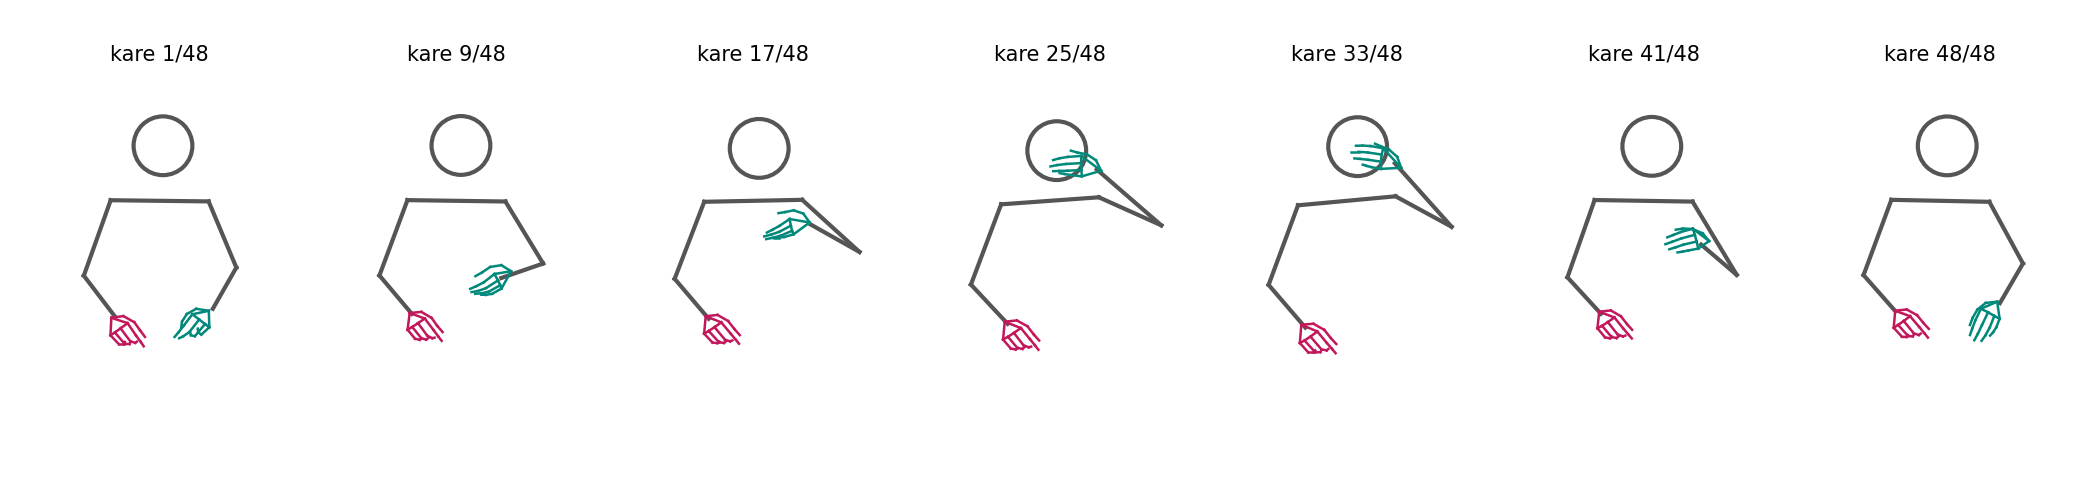
\includegraphics[width=\textwidth]{grafik/ornek_hareket.png}
\caption{\sol çorba\sag{} işaretinin örnek hareketinden kareler (eğitim kümesinden, normalize edilmiş noktalar)}
\label{fig:ornekhareket}
\end{figure}

\subsection{Sürekli tanıma}

Sürekli modda işaretin nerede başlayıp bittiğini bulmak için basit bir kural
kullanılmaktadır (\texttt{SegmentTracker}). En az bir elin bileği omuz ortasının bir
omuz genişliği altından yukarıdaysa kare \sol etkin\sag{} sayılır. Art arda iki etkin
kare görülünce bölüt açılır ve öncesindeki 8 kare başa eklenir; 600 ms boyunca etkinlik
olmazsa ya da 6 saniye dolarsa bölüt kapanıp sınıflandırılır. 12 kareden kısa bölütler
atılır. AUTSL test videoları 10 FPS'e seyreltilip bu kuralla bölütlendiğinde bulunan
bölütlerde doğruluk yüzde 89--90 olarak ölçülmüştür (\texttt{tune\_segmentation.py}).

\subsection{Gönüllü testi ekranı}

Gerçek ortam doğruluğunu ölçmek için uygulamaya ayrı bir test ekranı eklenmiştir.
Katılımcıya rastgele seçilmiş 10, 20 ya da 30 kelime sırayla gösterilir; her kelimenin
örnek hareketi ekranın üstünde oynar. Katılımcı işareti kaydeder, tahmin ve ilk üç aday
gösterilir. Her deneme yalnızca nokta koordinatları ve tahminle birlikte telefona JSON
olarak yazılır; kamera görüntüsü saklanmaz. Test sonunda Top-1, Top-3 ve eşiği geçenlerde
doğruluk özetlenir. Kayıtlar bilgisayara alınıp \texttt{live\_analysis.py} ile
incelenmektedir: betik kayıtları Python'da yeniden sınıflandırır, katılımcı bazında
doğruluk çıkarır ve canlı kayıtları AUTSL ile kare sayısı, elin görünme oranı,
kameraya uzaklık ve el hızı açısından karşılaştırır.

\subsection{Gizlilik ve çevrimdışı çalışma}

Uygulamanın Android bildiriminde (\textit{manifest}) yalnızca kamera izni
bulunmaktadır; internet izni yoktur. Model, MediaPipe dosyaları ve örnek hareketler
uygulama paketinin içindedir. Kamera görüntüsü hiçbir aşamada diske yazılmaz ve
cihazdan çıkmaz.

\subsection{Karşılaşılan sorunlar}

\begin{itemize}
  \item Yayın (\textit{release}) derlemesinde kod küçültme aracı (R8), MediaPipe'ın
        kullandığı protobuf alan adlarını değiştirdiği için uygulama açılışta
        çökmüştür. Yayın derlemesinde küçültme kapatılarak sorun giderilmiştir.
  \item Flutter'ın 3.50 sürümü projenin Gradle yapılandırmasıyla uyumsuz olduğu için
        Flutter 3.44.8 sürümüne sabitlenmiştir.
  \item Uzun video testleri ve sürekli kamera kullanımı orta segment telefonu
        ısıtmaktadır (46,7 °C ölçülmüştür). Bu nedenle CPU modu uzun süreli kullanım
        için önerilmemektedir.
\end{itemize}
